\section{Motivations for Next Generation CSACs}

\begin{frame}{Limitations of current CSACs}

    Current CSACs struggle to have short-term stability $\sigma_y(\tau) < 10^{-11}$ and long-term stability comparable with the one of CBT\footnotemark[1] clocks.

    \begin{columns}[c, onlytextwidth]

        \begin{column}{0.48\textwidth}

            \begin{figure}
                \centering
                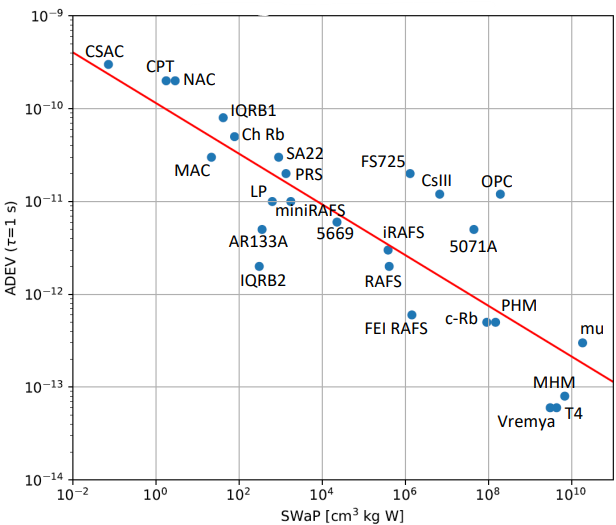
\includegraphics[height=0.4\textheight]{img/ADEV-vs-SWaP.png}
                \caption{Allan deviation vs. Size, Weight and Power of different atomic clocks.}
            \end{figure}

        \end{column}

        \hfill

        \begin{column}{0.48\textwidth}

            \begin{figure}
                \centering
                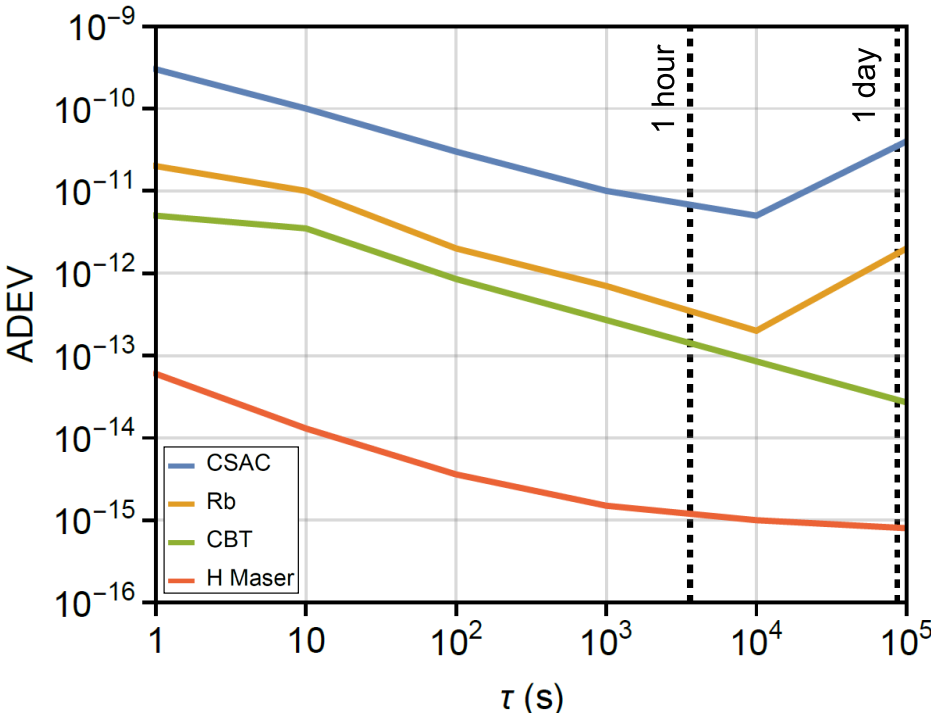
\includegraphics[height=0.4\textheight]{img/allan-without-quartz.png}
                \caption{Short and medium term stability of different atomic clocks.}
            \end{figure}

        \end{column}

    \end{columns}

    \textbf{Next generation of CSACs (NG-CSACs) has to exploit different physics.}

    \footnotetext[1]{CBT: Cesium Beam Tube}

\end{frame}



\begin{frame}{DARPA IMPACT \& ACES programs}

    DARPA\footnotemark[1] is again the main driver for the development of NG-CSACs.

    \vspace{10pt}

    \begin{columns}[c, onlytextwidth]

        \begin{column}{0.5\textwidth}

            Funded projects include:

            \begin{itemize}
                \item IMPACT\footnotemark[2]: $20cm^3$, $250mW$ with $\sigma_y(\tau=1month) < 160ns$.
                \item ACES\footnotemark[3]: palm sized, battery powered with $1000x$ performance improvements.
                \item ROCkN\footnotemark[4]: continuing of the ACES program.
            \end{itemize}

        \end{column}

        \hfill

        \begin{column}{0.45\textwidth}

            \begin{figure}
                \centering
                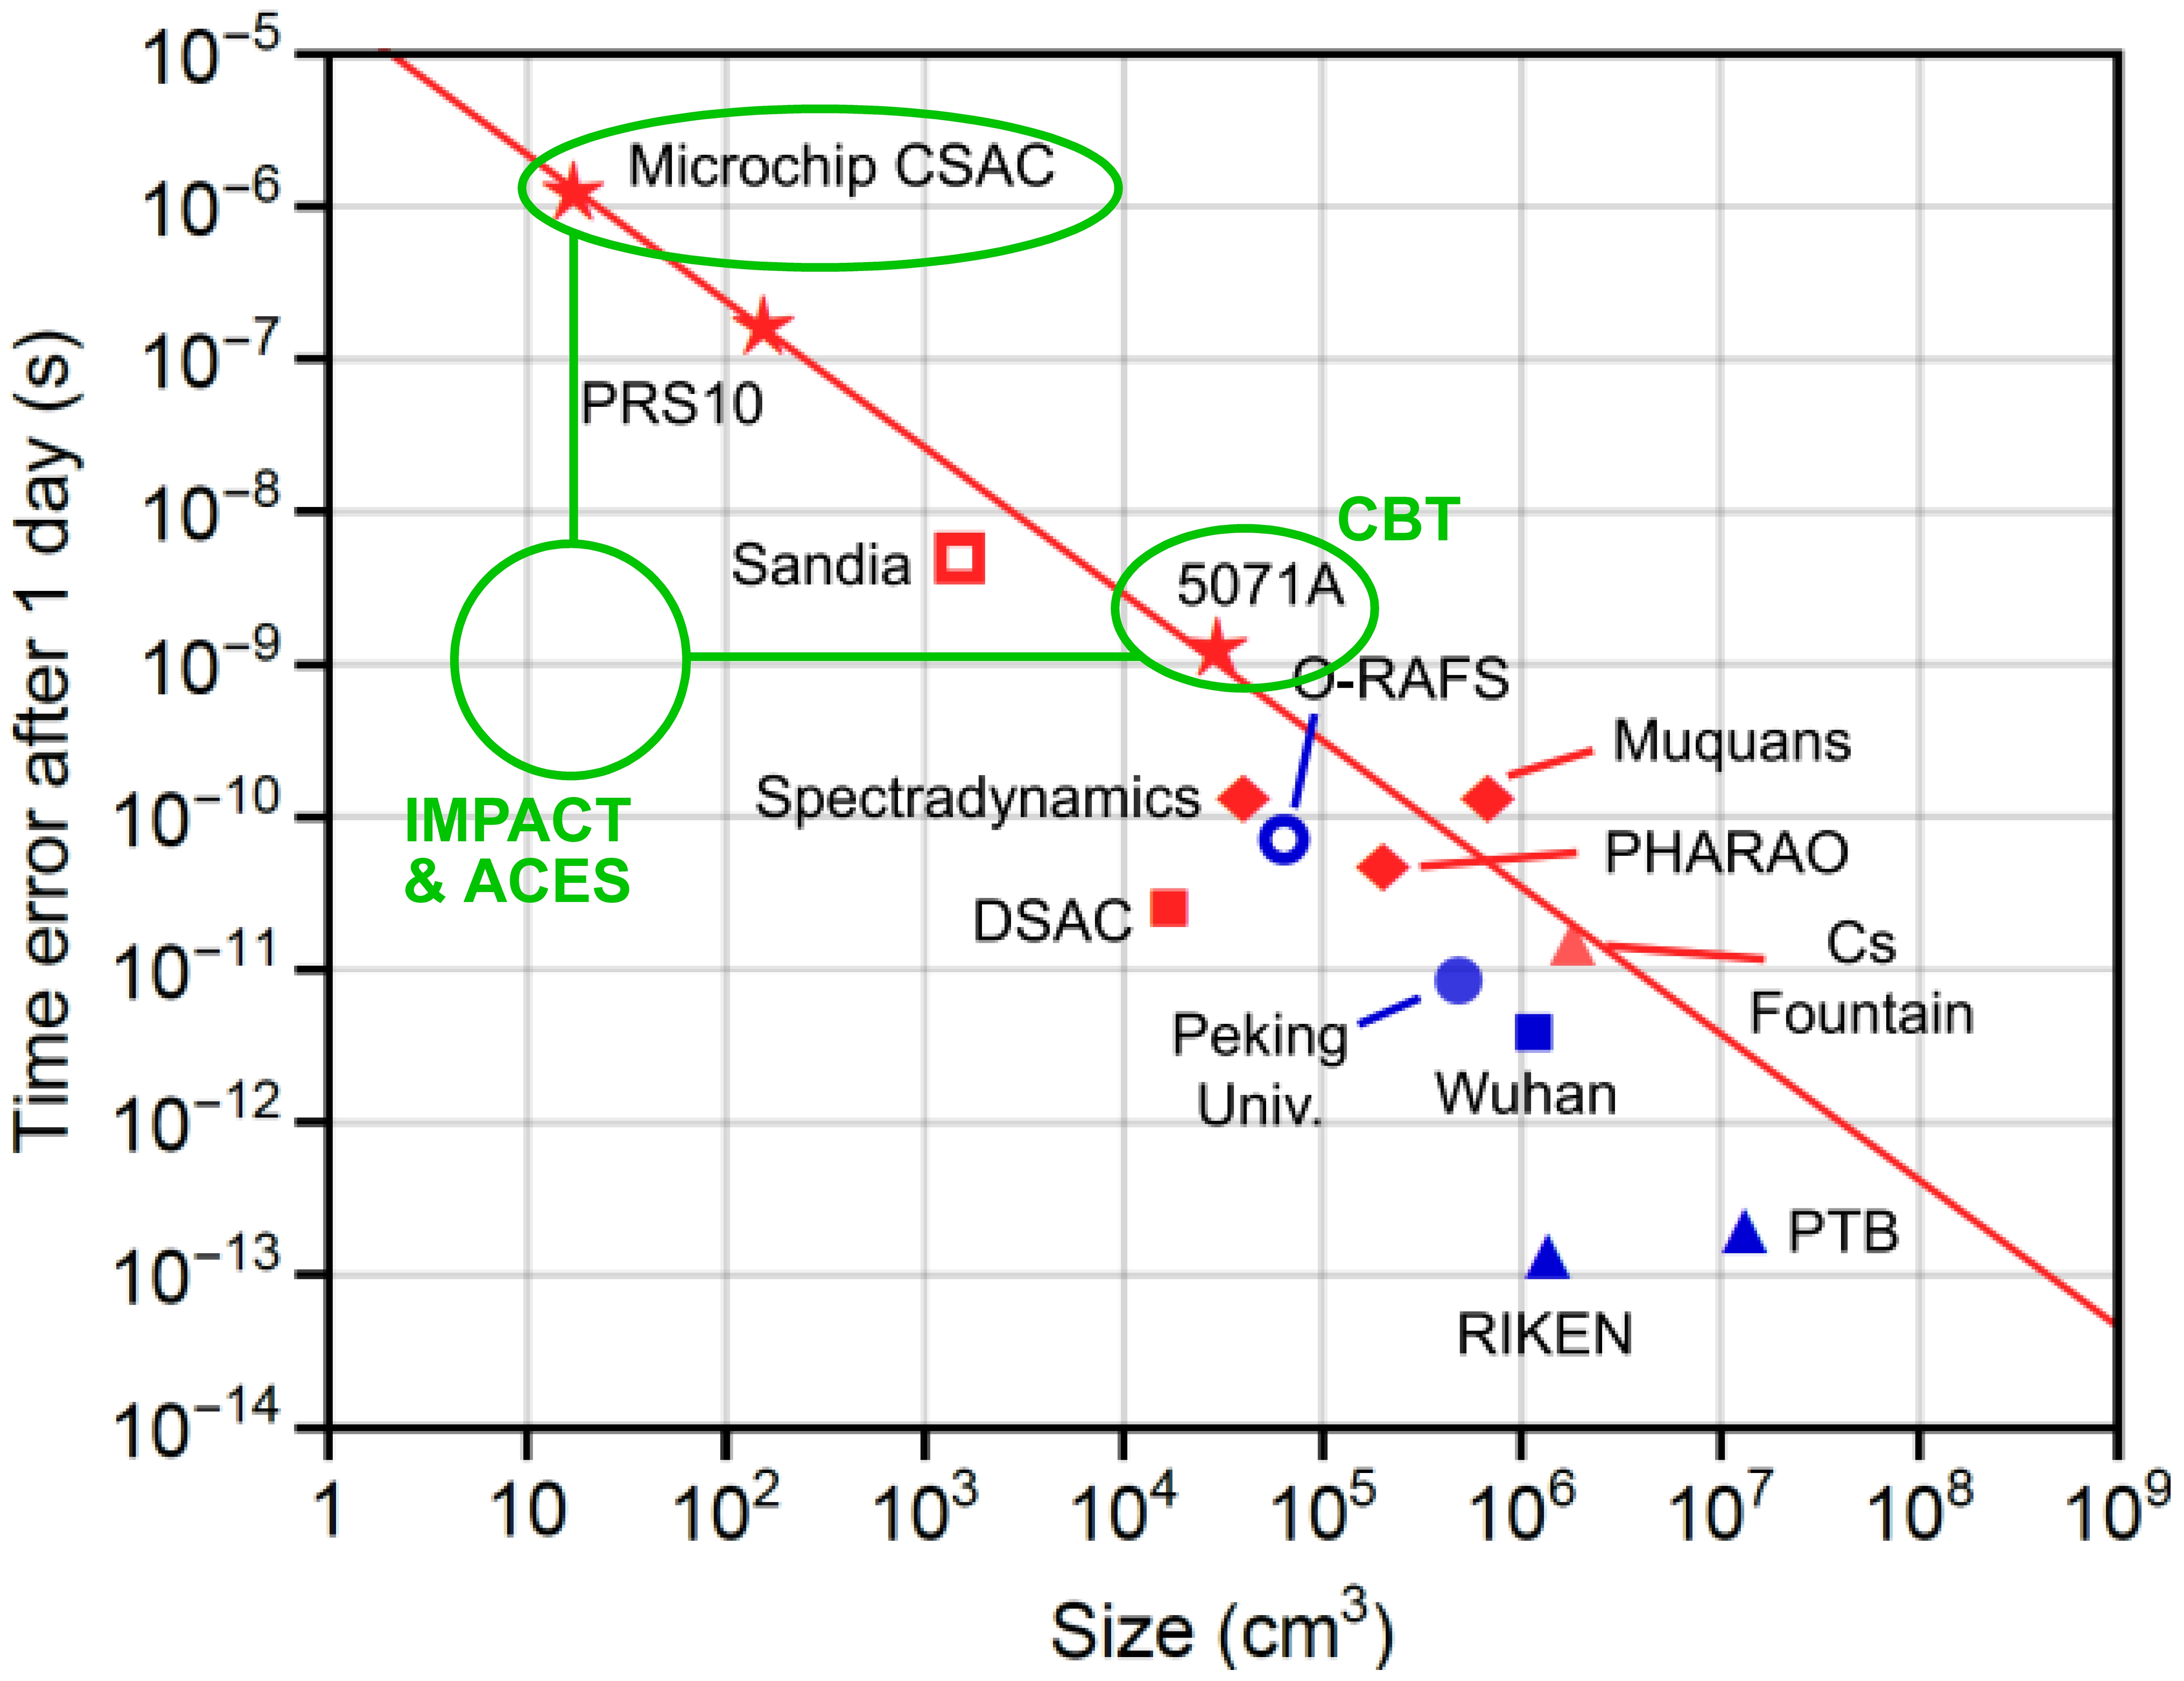
\includegraphics[width=\textwidth]{img/DARPA-stability-target.jpg}
                \caption{Programs' stability targets.}
            \end{figure}

        \end{column}

    \end{columns}

    \footnotetext[1]{DARPA: Defense Advanced Research Projects Agency.}
    \footnotetext[2]{IMPACT: Integrated Miniature Primary Atomic Clock Technology (2009-2015).}
    \footnotetext[3]{ACES: Atomic Clock with Enhanced Stability (2015-2022).}
    \footnotetext[4]{ROCkN: Robust Optical Clock Network (2022-ongoing).}

\end{frame}